\section{Appendix 1: Crossing Muons} \label{appendix:CrossingMuon}
Particles with energies higher than $\approx$ 150 MeV can cross the TPC volume and exit the TPC without experiencing an interaction. We define as “crossing” each particle that exits the TPC fiducial boundaries.\\
These particles will then contribute only in filling the $N_{incident}$ histogram for each point of their track, meaning that for the energies related to the track points they are more likely to survive than to interact with Ar nuclei.\\

The percentage of crossing tracks from the Closed Box data sample are reported in Tab.\ref{tabellaCrossing}. In Fig.\ref{CrossingOBKinEn} the Incident and Final kinetic energy of crossing tracks in the Open Box sample is reported.
\begin{table}[ht!]
\centering
\begin{tabular}{|c|c|}
\hline
\textbf{Event Sample} & \textbf{Number of Events} \\ 
\hline \hline
Run I Negative Polarity Data Sample                                                                          & 486753           \\
\hline
After all selection cuts                                                                      & 2404             \\
\hline
Crossing tracks                                                                               & 858              \\
\hline
\% Crossing tracks over events that pass all cuts & 35.7 \%\\          
\hline
\end{tabular}
\caption{Crossing tracks after all the selection cuts for a subsample of Run-I data.} 
\label{tabellaCrossing}
\end{table}

\begin{figure}[h!]
\centering
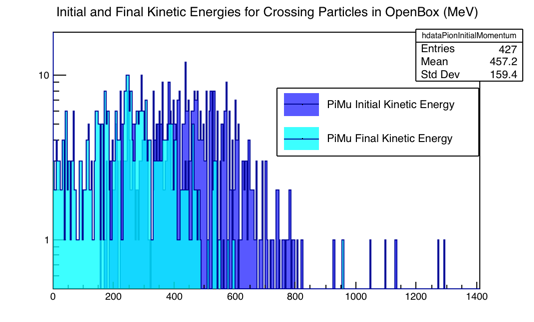
\includegraphics[scale=0.45]{./images/OBparticles_crossingKinEn.png}
\caption{Initial and Final kinetic energy spectra for Crossing tracks ifor a subsample of Run-I data.}
\label{CrossingOBKinEn}
\end{figure}

We know the particles from the beamline which can exit the TPC boundaries will be mainly pions and muons. It is then natural to evaluate the percentage of contamination by muons in our "crossing particles" data sample. Since crossing muon tracks will be taken into account when filling the $N_{incident}$ histogram for the Pion cross section evaluation. The {\textbf{crossing muon contamination}} in $N_{incident}$ will then affect our measurement.

We agreed to provide an estimate for the contribution of "crossing muon" events via Monte Carlo simulation. We will then apply this "crossing muon contamination" correction on the $N_{incident}$ histogram made from the data sample.\\
We made a study of crossing track events from the MC sample of pions and muons (the incoming particles energy spectrum was re-weighted based on the beam profile). In Tab.\ref{tab:CrossingMC} we show the percentages of crossing pions and muons after our selection cuts, in case a fixed number of pions and muons are shot in our MC simulation. Muons are not strongly affected by our selection cuts and we see they're mostly crossing events (almost 76\% of the selected muon events are crossing tracks). Pion statistic is a bit more affected by our cuts than the muon's: 70.1\% of the pions that enter the TPC made it to pass all our selection cuts and only 32\% of them are crossing tracks, since most of them interact into the TPC volume.\\
% Considering crossing events, from Tab.\ref{tab:CrossingMC} we see:
% $$ \Big(\frac{\mu}{\pi}\Big)_{cross,cuts}^{MC, unweighted} \simeq 3 $$
% this is in case of same number of pions and muons shot via MC.
For our analysis, it is important to consider the relative fraction of pions and muons in the beam to get a proper estimate of the real crossing muon contamination of our sample. The muon to pion fraction from the beam composition is, for negative polarity runs (See Tab.\ref{tab:beamcomp1}): 
$$ \Big(\frac{\mu}{\pi}\Big)_{beam} \simeq 0.045 $$
%commented stuff - weird results - to be updated soon
Therefore if we weight by the beam composition the crossing muons to crossing pions ratio obtained before, we can get an average estimate over all energies for the $(\frac{\mu}{\pi})_{cross}$ we can expected in the Data:
$$ \Big(\frac{\mu}{\pi}\Big)_{cross,cuts}^{MC, weighted} \simeq  0.136 $$
The average MC estimate of the composition of Crossing Tracks sample is then: 88\% pions, 12\% muons.\\ 
% (on average - MC estimate): 
% Pi: 88 %
% Mu: 12 %
% (considering the beam composition and assuming ONLY Pi and Mu cross the TPC)

A more complete analysis has been made considering the crossing muon contamination in each energy bin of $N_{incident}$ histogram, as shown in Fig.\ref{CrossingMCNinc}, Fig.\ref{CrossingOBMuon} and Fig.\ref{CrossingFraction}. \\
The fraction of crossing muons in each energy bin of $N_{incident}$ histogram will actually make our denominator for cross section calculation higher then if we had only pions.
From the plot in Fig.\ref{CrossingFraction} we see the fractional contribution of crossing muons is quite flat, at least in the 50-650 MeV region.
We have decided to consider a uniform crossing muon contamination factor of the order of 10\% and to apply this correction in each energy bin of the $N_{incident}$ histogram made from our Data sample. This results in a 9\% reduction of the content of each energy bin. We will also assume a 20\% uncertainty on our estimate of the crossing muon contamination factor in $N_{incident}$, that will reflect in a $\approx$ 3\% systematic on the cross section measurement for each energy bin.

$$ N_{incident}^{data} \longrightarrow N_{incident}^{data, \mu corr} \text{ applied 9\% crossing $\mu$ contamination correction}$$
$$\sigma \approx \frac{N_{incident}^{data}}{N_{incident}^{data, \mu corr}} \text{ , } \Big(\frac{\Delta\sigma}{\sigma}\Big)_{sys}^{\mu corr} \simeq 3 \% $$ 


\begin{table}[ht!]
\centering
\begin{tabular}{|l|l|l|}
\hline
\textbf{Event Sample}                                                                                 & {\textbf{Pions}} & {\textbf{Muons}} \\ \hline \hline
MC sample                                                                                     & 118800 & 79200 \\ \hline
MC sample - particles that enter the TPC                                                      & 80603 & 76328 \\ \hline
After all selection cuts                                                                      & 56462 & 63146 \\ \hline
Crossing tracks                                                                               & 26035  & 58261 \\ \hline
\% Crossing tracks  & 32.3 \% & 76.3 \% \\ \hline
\end{tabular}
\caption{Crossing tracks after all the selection cuts for pions and muons (from MC).}
\label{tab:CrossingMC}
\end{table}


% \begin{figure}[h!]
% \begin{minipage}{0.5\textwidth}
% 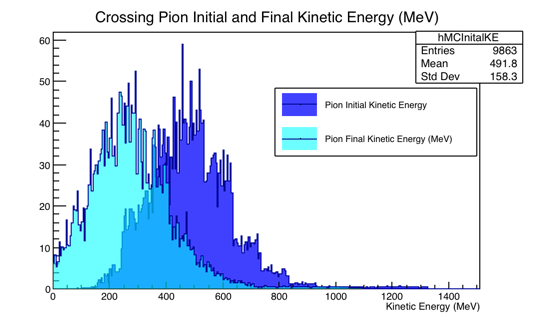
\includegraphics[width=\textwidth]{PionCrossingKinEn.png}
% \end{minipage}
% \begin{minipage}{0.5\textwidth}
% 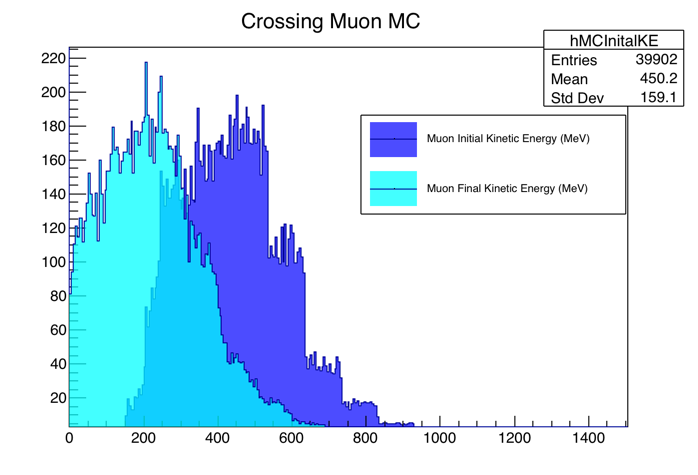
\includegraphics[width=\textwidth]{CrossMuKinEn.png}
% \end{minipage}
% \caption{Initial and Final kinetic energy spectra for Crossing Pion and Muon tracks from MC Sample.}
% \label{CrossingMCPionKinEn}
% \end{figure}

% \begin{figure}[h!]
% \centering
% 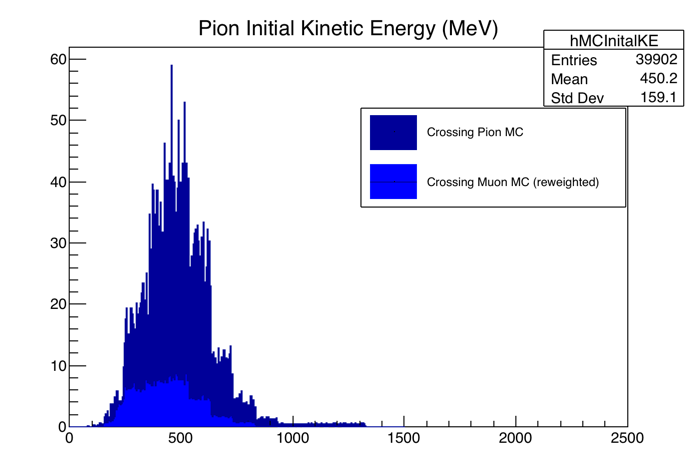
\includegraphics[scale=0.4]{CrossMuPiKinEn.png}
% \caption{Initial kinetic energy spectra for Crossing Pion and Muon tracks from MC Sample weighted by beam composition.}
% \end{figure}

\begin{figure}[h!]
\begin{minipage}{0.5\textwidth}
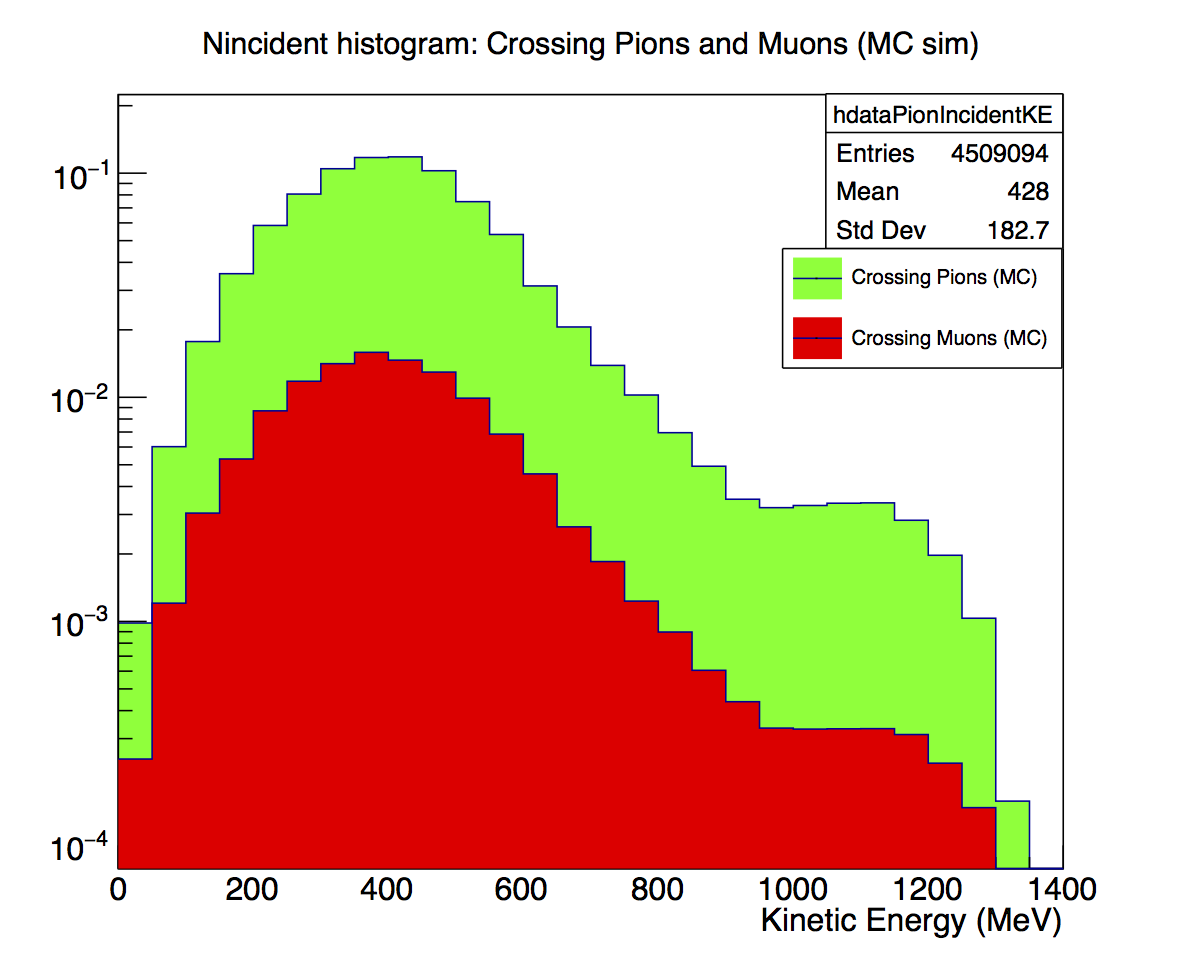
\includegraphics[width=\textwidth]{./images/CrossingPiMu.png}
\end{minipage}
\begin{minipage}{0.5\textwidth}
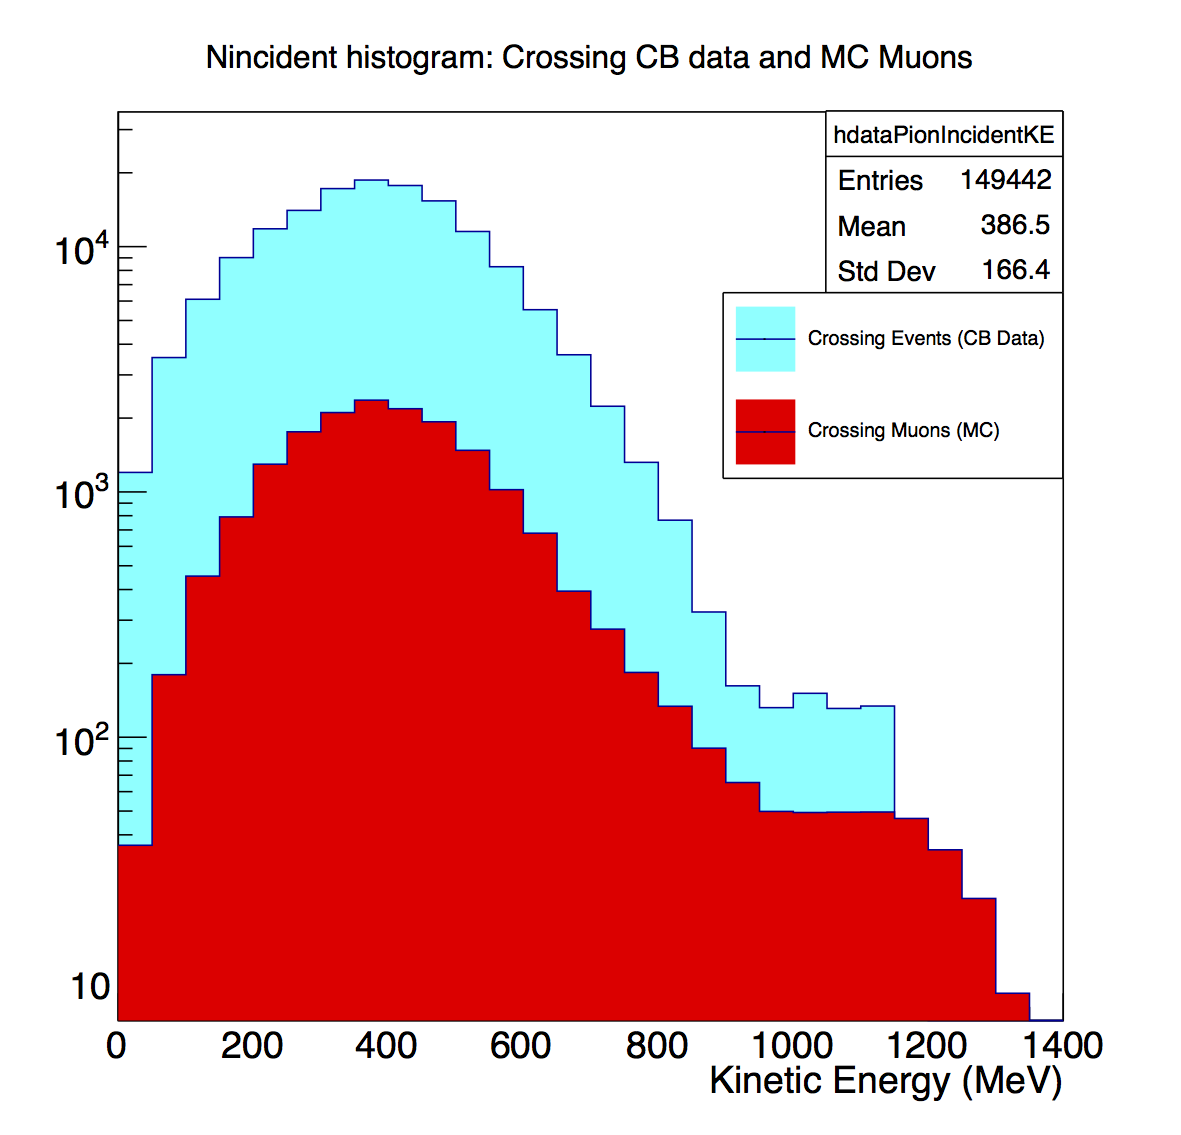
\includegraphics[width=\textwidth]{./images/CrossingCBandMuMC.png}
\end{minipage}
\caption{$N_{incident}$ histogram for Crossing Pion and Muon tracks from MC Sample weighted by muon to pion ratio from the beam composition. (The histogram is normalized to the sum of crossing Muons and crossing Pions statistic - the total of crossing events).[left] $N_{incident}$ histogram for Run I Neg.Pol. Data sample (CB) Crossing Events and for Crossing Muon tracks from MC Sample.[right]}
\label{CrossingMCNinc}
\end{figure}

\begin{figure}[h!]
\centering
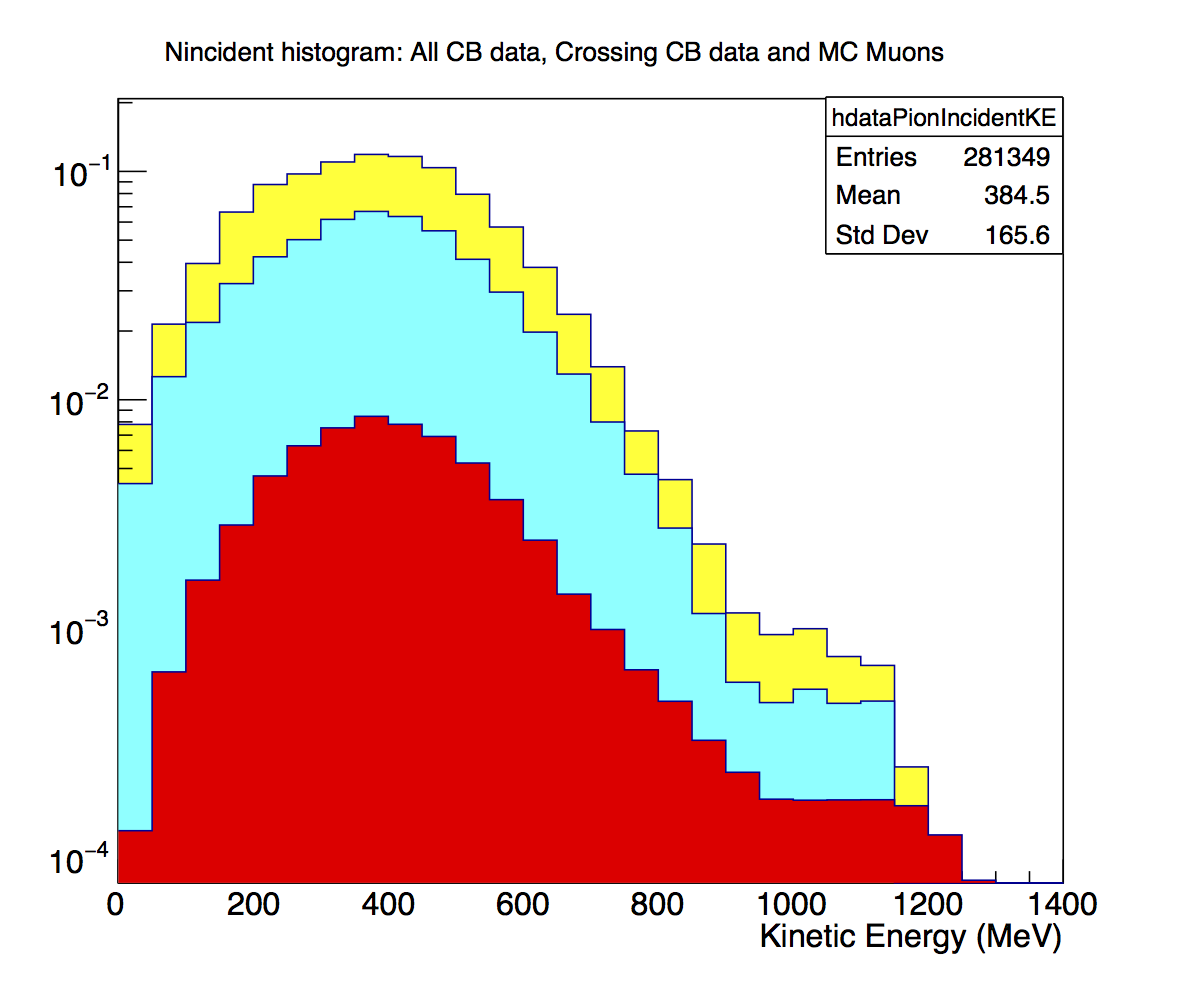
\includegraphics[scale=0.5]{./images/CBAllandCross_CrossMuMC.png}
\caption{$N_{incident}$ histogram for for a subsample of Run-I data (All [yellow] and only crossing [cyan]) and for Crossing Muon tracks from MC Sample [red]. (The histograms are normalized to the the data statistic in $N_{incident}$.)}
\label{CrossingOBMuon}
\end{figure}

\begin{figure}[h!]
\centering
%\includegraphics[scale=0.4]{./images/CrossMu_FractionOK.pdf}
\caption{Crossing Muon fraction on for a subsample of Run-I data in $N_{incident}$ histogram. }
\label{CrossingFraction}
\end{figure}
